
  \subsubsection{Back-end}
  \paragraph{Informazioni sul package} 
    \begin{figure}[H] 
      \begin{center} 
        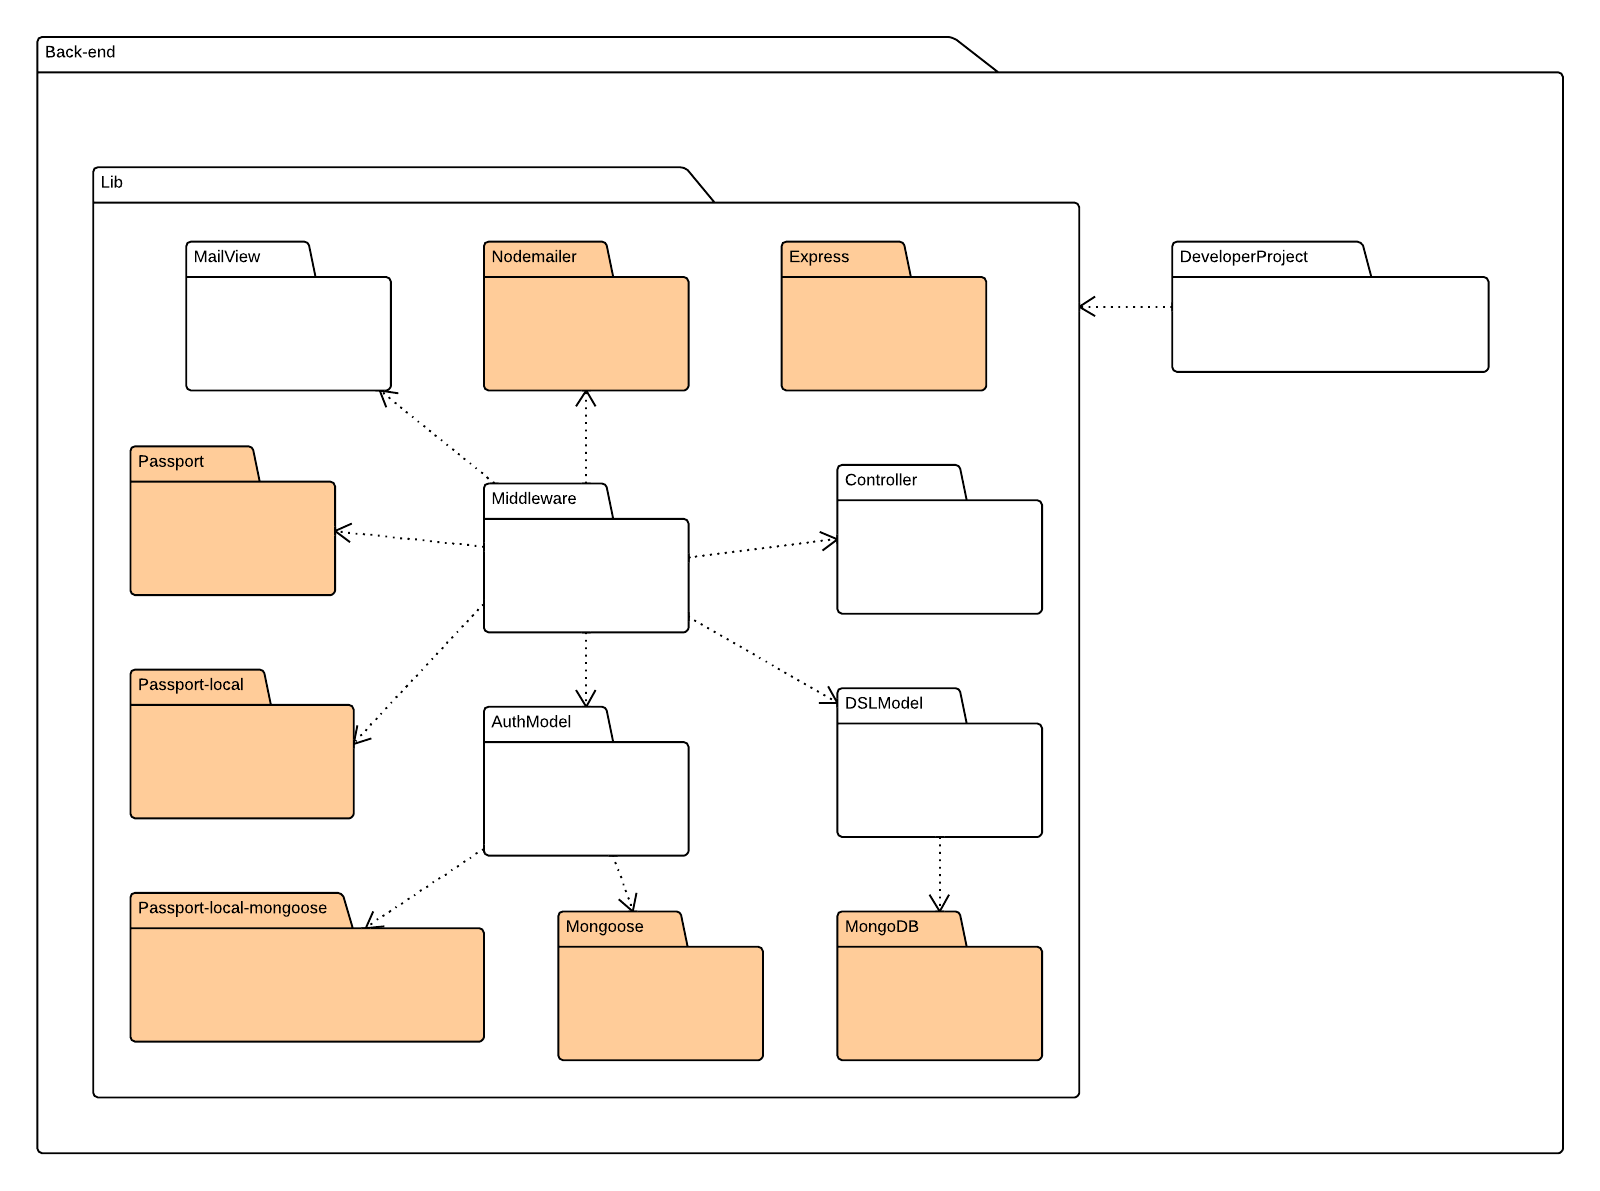
\includegraphics[width=\textwidth]{packages/Back-end.png}  
        \caption{Componente Back-end}
      \end{center}  
    \end{figure} 
  \subparagraph{Descrizione} 
    \begin{itemize}
    \item[] 
    \end{itemize} 
    \subparagraph{Package contenuti} 
    \begin{itemize}
        \item Back-end::DeveloperProject
        \item Back-end::Lib
    \end{itemize}
  \subsubsection{Back-end::Lib::AuthModel}
  \paragraph{Informazioni sul package} 
    \begin{figure}[H] 
      \begin{center} 
        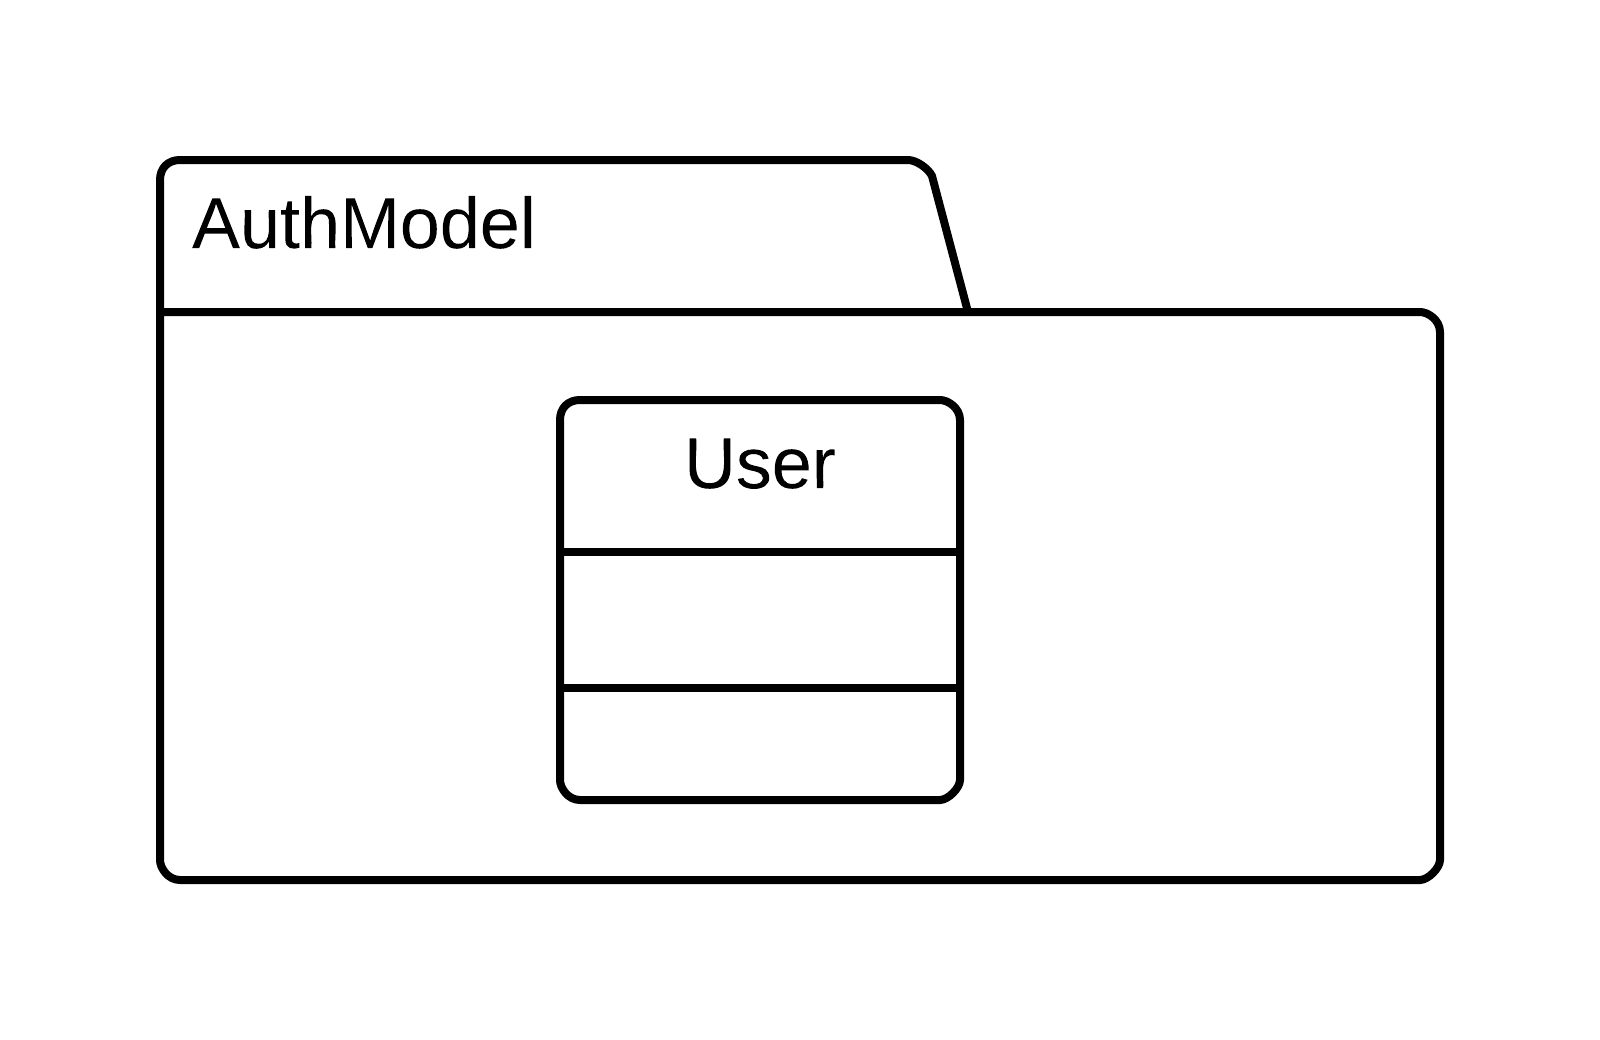
\includegraphics[width=\textwidth]{packages/Back-end::Lib::AuthModel.png}  
        \caption{Componente Back-end::Lib::AuthModel}
      \end{center}  
    \end{figure} 
  \subparagraph{Descrizione} 
    \begin{itemize}
    \item[] \glossario{Package} che gestisce i dati e le operazioni relativi all'autenticazione utente, andando ad aggiungersi alle componenti che compongono la parte model nell'architettura MVC nel back-end. 
    \end{itemize} 
    \paragraph{Classi}
      \subparagraph{Back-end::Lib::AuthModel::User}
        
        \textbf{\\ \\ Descrizione} 
          \begin{itemize}
            \item[] Classe che si occupa dei metodi per la gestione dei dati utente. 
          \end{itemize}      
        \textbf{Utilizzo}  
          \begin{itemize}
            \item[] Viene utilizzata per l'interfacciamento con la libreria \glossario{Mongoose} per la registrazione dello schema dei dati, e con la libreria passport-local-mongoose per il popolamento automatico dello schema con campi dati e metodi predefiniti.
Il costruttore del modello dello schema dei dati viene registrato nella \glossario{Factory} di \glossario{Mongoose} ed ogni istanza condividerà la stessa connessione al server.
          \end{itemize}
  \subsubsection{Back-end::DeveloperProject}
  \paragraph{Informazioni sul package} 
    \begin{figure}[H] 
      \begin{center} 
        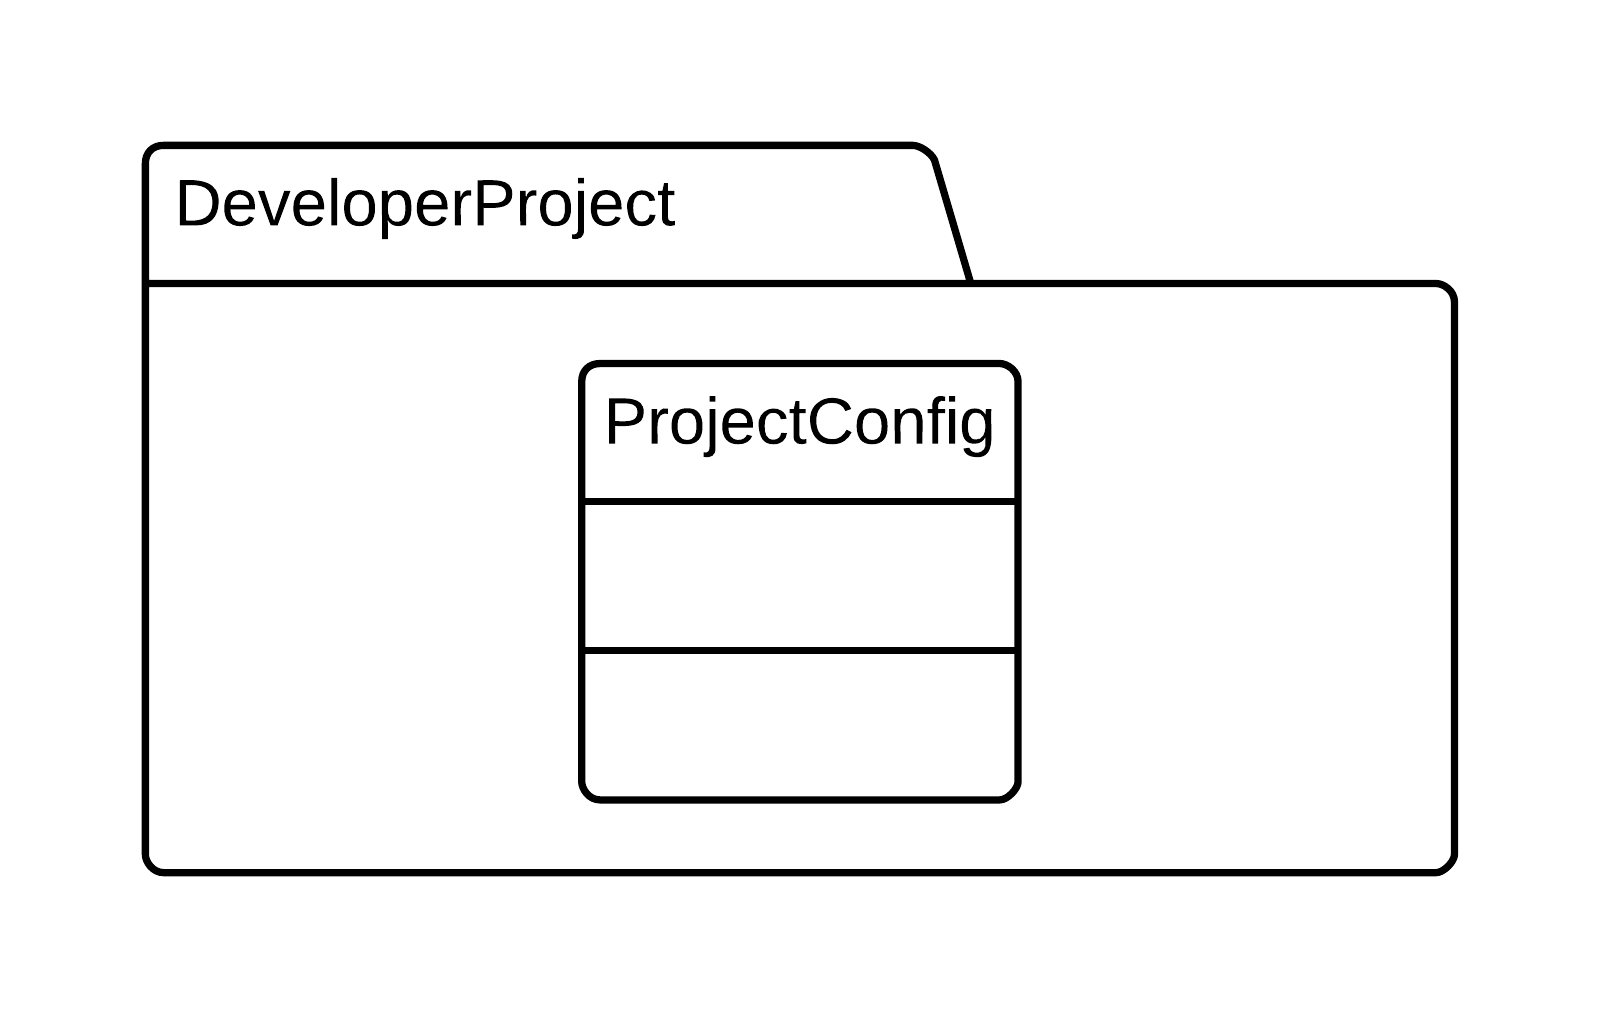
\includegraphics[width=\textwidth]{packages/Back-end::DeveloperProject.png}  
        \caption{Componente Back-end::DeveloperProject}
      \end{center}  
    \end{figure} 
  \subparagraph{Descrizione} 
    \begin{itemize}
    \item[] 
    \end{itemize} 
    \paragraph{Classi}
      \subparagraph{Back-end::DeveloperProject::ProjectConfig}
        
        \textbf{\\ \\ Descrizione} 
          \begin{itemize}
            \item[] Classe che si occupa di configurare il progetto creato dallo sviluppatore.
          \end{itemize}      
        \textbf{Utilizzo}  
          \begin{itemize}
            \item[] Viene utilizzata per descrivere tutti i parametri dell'applicazione. Quando viene creata una \texttt{Back-end::Lib::ServerApp} le viene passato un oggetto di questo tipo ed essa avvierà l'applicazione a partire da questa configurazione.
          \end{itemize}
  \subsubsection{Back-end::Lib::MailView}
  \paragraph{Informazioni sul package} 
    \begin{figure}[H] 
      \begin{center} 
        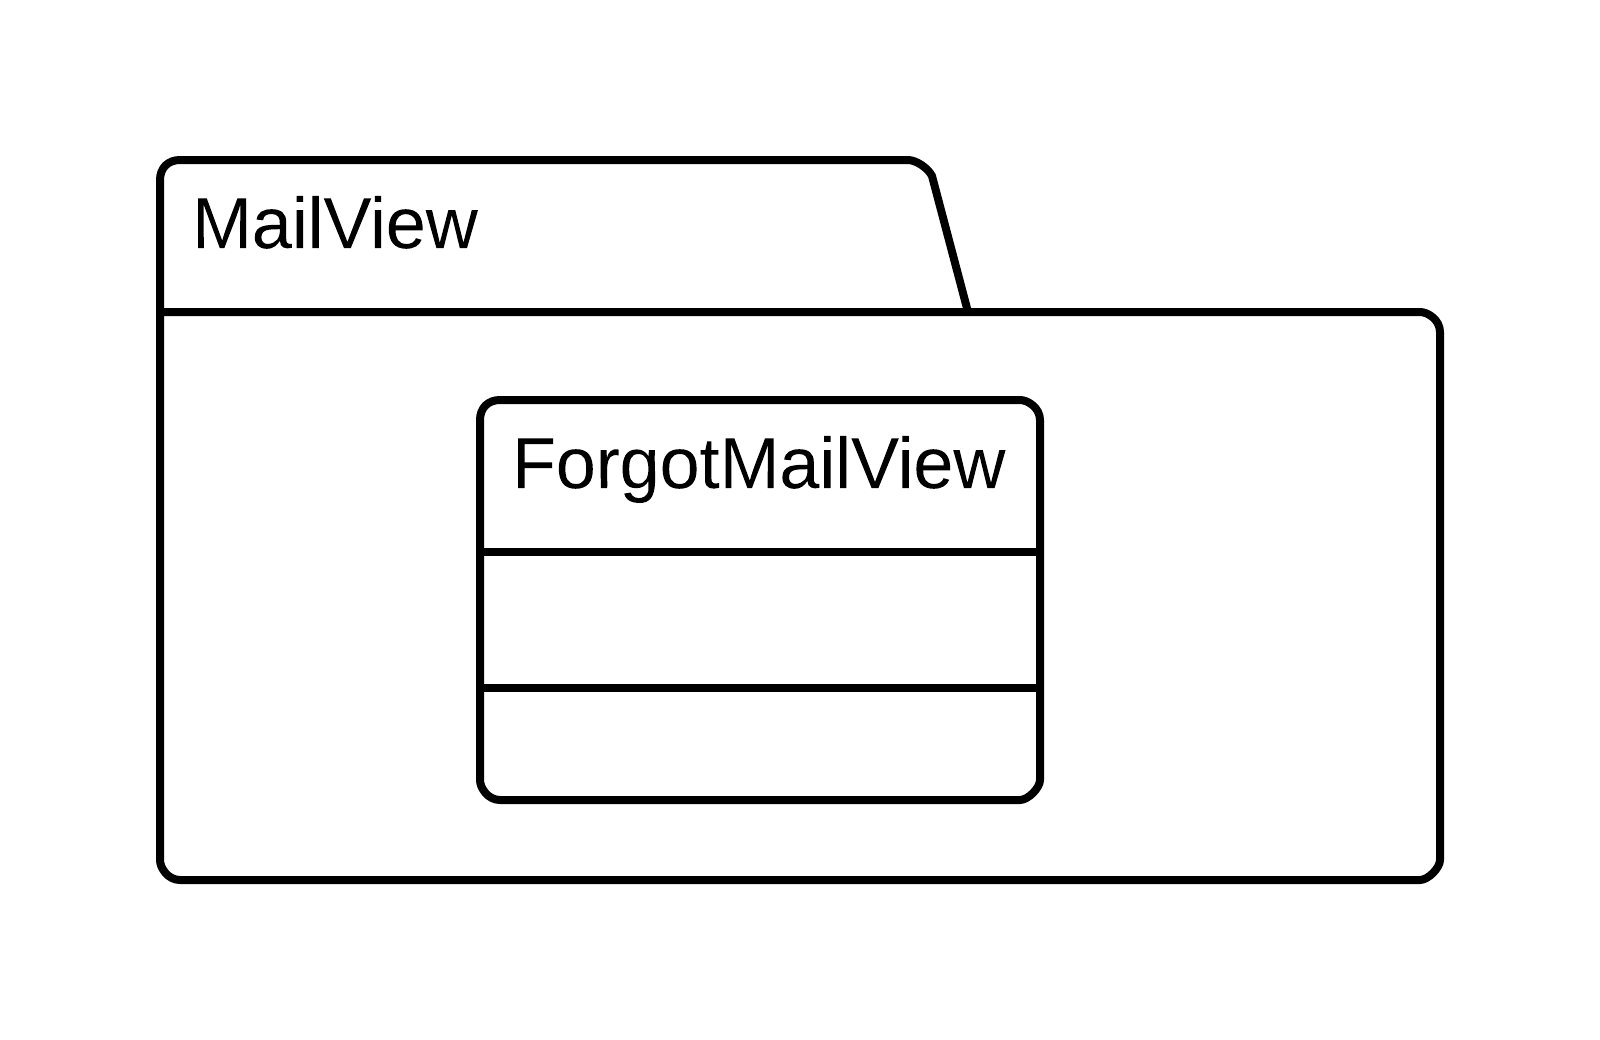
\includegraphics[width=\textwidth]{packages/Back-end::Lib::MailView.png}  
        \caption{Componente Back-end::Lib::MailView}
      \end{center}  
    \end{figure} 
  \subparagraph{Descrizione} 
    \begin{itemize}
    \item[] 
    \end{itemize} 
    \paragraph{Classi}
      \subparagraph{Back-end::Lib::MailView::ForgotMailView}
        
        \textbf{\\ \\ Descrizione} 
          \begin{itemize}
            \item[] Classe che fornisce una rappresentazione della mail.
          \end{itemize}      
        \textbf{Utilizzo}  
          \begin{itemize}
            \item[] Viene utilizzata come template di email da inviare nel caso in cui l'utente richieda il recupero password.
          \end{itemize}
  \subsubsection{Back-end::Lib}
  \paragraph{Informazioni sul package} 
    \begin{figure}[H] 
      \begin{center} 
        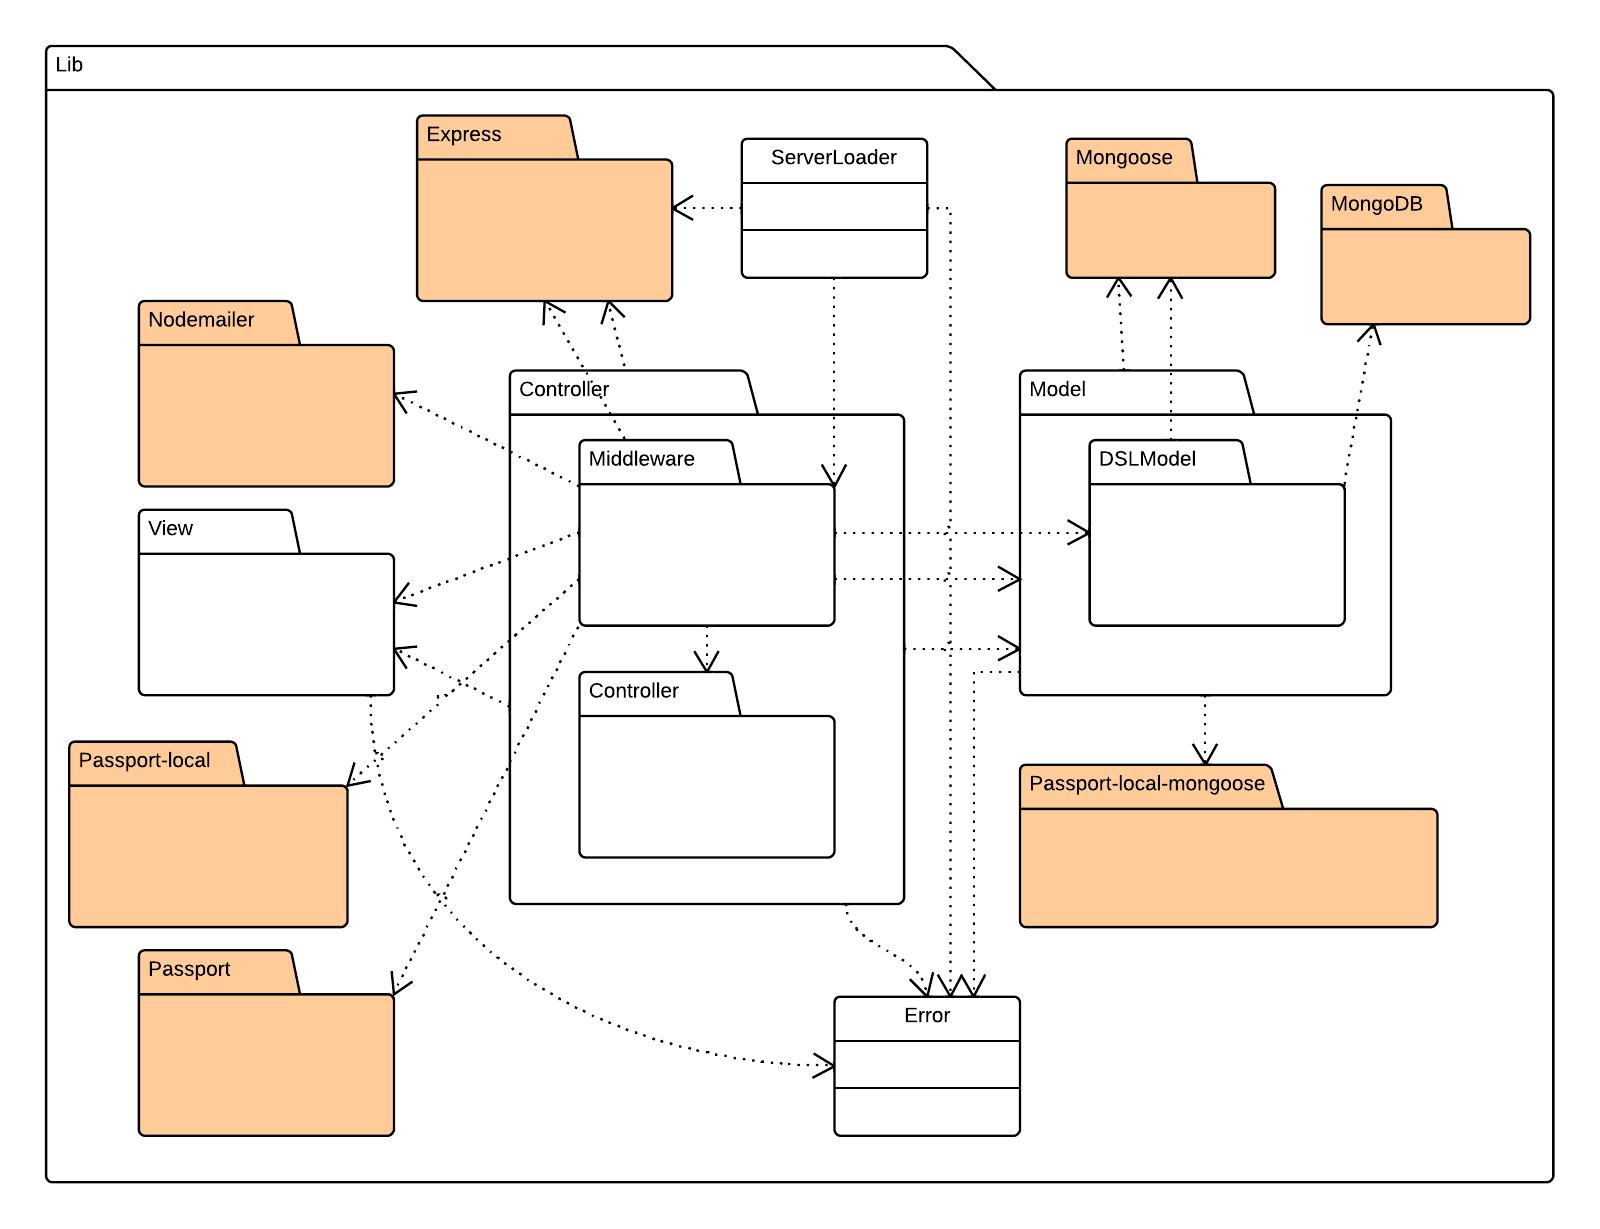
\includegraphics[width=\textwidth]{packages/Back-end::Lib.png}  
        \caption{Componente Back-end::Lib}
      \end{center}  
    \end{figure} 
  \subparagraph{Descrizione} 
    \begin{itemize}
    \item[] 
    \end{itemize} 
    \subparagraph{Package contenuti} 
    \begin{itemize}
        \item Back-end::Lib::AuthModel
        \item Back-end::Lib::MailView
        \item Back-end::Lib::Middleware
        \item Back-end::Lib::DSLModel
        \item Back-end::Lib::Controller
    \end{itemize}
  \subsubsection{Back-end::Lib::Middleware}
  \paragraph{Informazioni sul package} 
    \begin{figure}[H] 
      \begin{center} 
        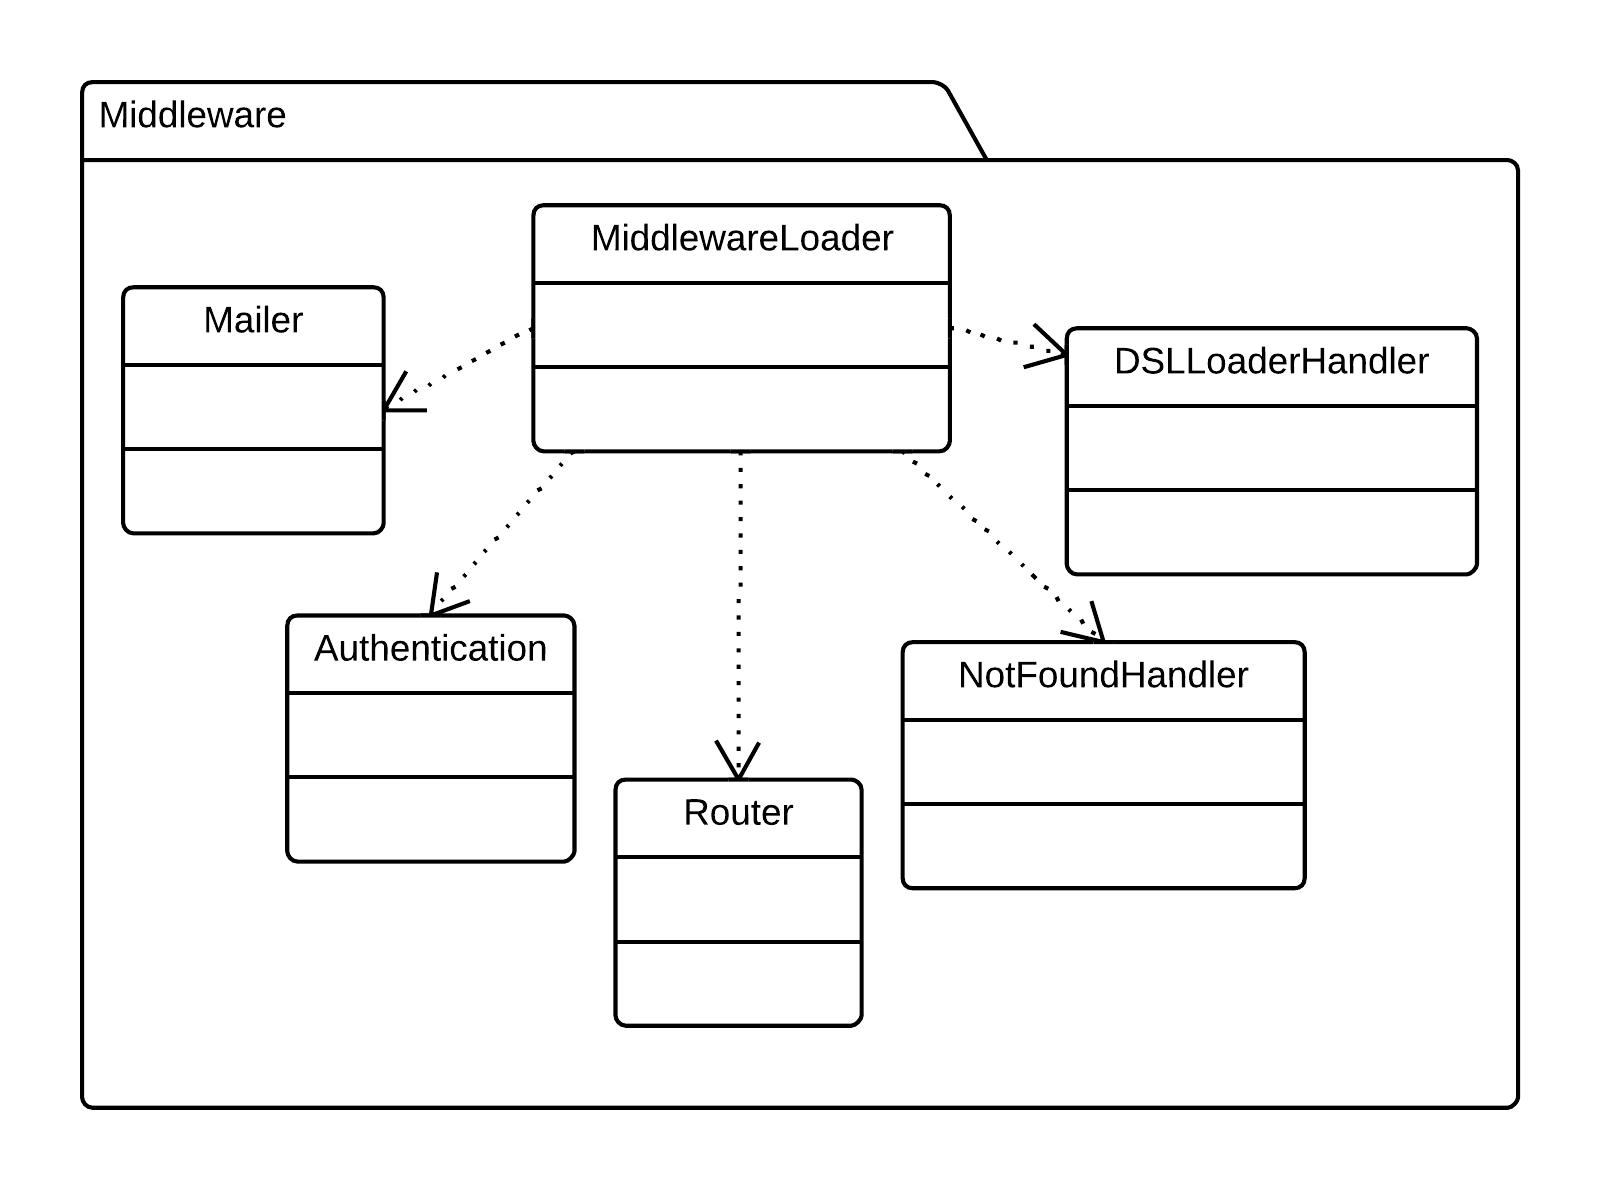
\includegraphics[width=\textwidth]{packages/Back-end::Lib::Middleware.png}  
        \caption{Componente Back-end::Lib::Middleware}
      \end{center}  
    \end{figure} 
  \subparagraph{Descrizione} 
    \begin{itemize}
    \item[] \glossario{Package} contenente classi che costituiscono gli handler della catena di chiamate a cui viene passata la responsabilità di gestire una richiesta,  decorando quest'ultima con parametri e metodi utilizzabili dai controller. Costituisce una parte dell' \glossario{application logic} nell'architettura mvc del back-end.
    \end{itemize} 
    \paragraph{Classi}
      \subparagraph{Back-end::Lib::Middleware::Router}
        
        \textbf{\\ \\ Descrizione} 
          \begin{itemize}
            \item[] Classe che si occupa della richiesta di risorse. È uno dei componenti subsystem class del \glossario{Design Pattern} \glossario{Facade} e handler del \glossario{Design Pattern} \glossario{Chain of responsability}.
          \end{itemize}      
        \textbf{Utilizzo}  
          \begin{itemize}
            \item[] Si occupa di smistare la richiesta in base all'\glossario{URI} ricevuto e ad invocare l'opportuno metodo di creazione sulla classe \texttt{Back-end::Lib::Controller::ControllerFactory}.
          \end{itemize}
      \subparagraph{Back-end::Lib::Middleware::Authentication}
        
        \textbf{\\ \\ Descrizione} 
          \begin{itemize}
            \item[] Classe che si occupa dell'autenticazione di un'utente. È uno dei componenti subsystem class del \glossario{Design Pattern} \glossario{Facade} e handler del \glossario{Design Pattern} \glossario{Chain of responsability}.
          \end{itemize}      
        \textbf{Utilizzo}  
          \begin{itemize}
            \item[] Viene utilizzata per verificare i dati inseriti dall'utente nella pagina di login e controllare l'effettiva corrispondenza delle credenziali nel \glossario{database}.
          \end{itemize}
          \textbf{Relazioni con altre classi}
          \begin{itemize}
              \item{Back-end::Lib::AuthModel::User}
          \end{itemize}
      \subparagraph{Back-end::Lib::Middleware::DSLLoaderHandler}
        
        \textbf{\\ \\ Descrizione} 
          \begin{itemize}
            \item[] Classe che si occupa di caricare i \glossario{DSL} presenti nel sistema. È uno dei componenti subsystem class del \glossario{Design Pattern} \glossario{Facade} e handler del \glossario{Design Pattern} \glossario{Chain of responsability}.
          \end{itemize}      
        \textbf{Utilizzo}  
          \begin{itemize}
            \item[] Viene utilizzata per caricare i \glossario{DSL} delle \glossario{Collection} all'interno del \glossario{database}.
          \end{itemize}
          \textbf{Relazioni con altre classi}
          \begin{itemize}
              \item{Back-end::Lib::DSLModel::DSLDomain}
          \end{itemize}
      \subparagraph{Back-end::Lib::Middleware::Mailer}
        
        \textbf{\\ \\ Descrizione} 
          \begin{itemize}
            \item[] Classe che si occupa dell'invio di email. È uno dei componenti subsystem class del \glossario{Design Pattern} \glossario{Facade} e handler del \glossario{Design Pattern} \glossario{Chain of responsability}.
          \end{itemize}      
        \textbf{Utilizzo}  
          \begin{itemize}
            \item[] Viene utilizzata per inviare un'email ad un utente che ha effettuato la richiesta di recupero password.
          \end{itemize}
          \textbf{Relazioni con altre classi}
          \begin{itemize}
              \item{Back-end::Lib::MailView::ForgotMailView}
          \end{itemize}
      \subparagraph{Back-end::Lib::Middleware::MiddlewareLoader}
        
        \textbf{\\ \\ Descrizione} 
          \begin{itemize}
            \item[] Classe che definisce un'interfaccia comune per tutte le richieste dell'applicazione. È la componente facade del \glossario{Design Pattern} \glossario{Facade} e handler del \glossario{Design Pattern} \glossario{Chain of responsability}.
          \end{itemize}      
        \textbf{Utilizzo}  
          \begin{itemize}
            \item[] Viene utilizzato per istanziare in modo "nascosto" all'applicazione tutti i \glossario{middleware} presenti nel componente \texttt{Back-end::Lib::Middleware}.
          \end{itemize}
          \textbf{Relazioni con altre classi}
          \begin{itemize}
              \item{Back-end::Lib::Middleware::Router}
              \item{Back-end::Lib::Middleware::Authentication}
              \item{Back-end::Lib::Middleware::DSLLoaderHandler}
              \item{Back-end::Lib::Middleware::Mailer}
              \item{Back-end::Lib::Middleware::NotFoundHandler}
          \end{itemize}
      \subparagraph{Back-end::Lib::Middleware::NotFoundHandler}
        
        \textbf{\\ \\ Descrizione} 
          \begin{itemize}
            \item[] Classe che si occupa la gestione dell'errore di pagina non trovata. È uno dei componenti subsystem class del \glossario{Design Pattern} \glossario{Facade} e handler del \glossario{Design Pattern} \glossario{Chain of responsability}.
          \end{itemize}      
        \textbf{Utilizzo}  
          \begin{itemize}
            \item[] Viene utilizzata per generare una pagina 404 di errore nel caso in cui l'\glossario{URI} passato non corrisponda ad una risorsa presente nell'applicazione.
          \end{itemize}
      \subparagraph{Back-end::Lib::Middleware::Errorhandler}
        
        \textbf{\\ \\ Descrizione} 
          \begin{itemize}
            \item[] Questa classe gestisce gli errori generati nei precedenti middleware o controller. Invia al client una risposta con stato HTTP 500 (server error) con una descrizione dell'errore nel formato JSON.
È uno dei componenti subsystem class del \glossario{Design Pattern} \glossario{Facade} e handler del \glossario{Design Pattern} \glossario{Chain of responsability}.
          \end{itemize}      
        \textbf{Utilizzo}  
          \begin{itemize}
            \item[] Questo middleware viene utilizzato per ultimo nella catena di gestione delle richieste di Express, in modo da gestire tutti gli errori generati precedentemente.
          \end{itemize}
  \subsubsection{Back-end::Lib::DSLModel}
  \paragraph{Informazioni sul package} 
    \begin{figure}[H] 
      \begin{center} 
        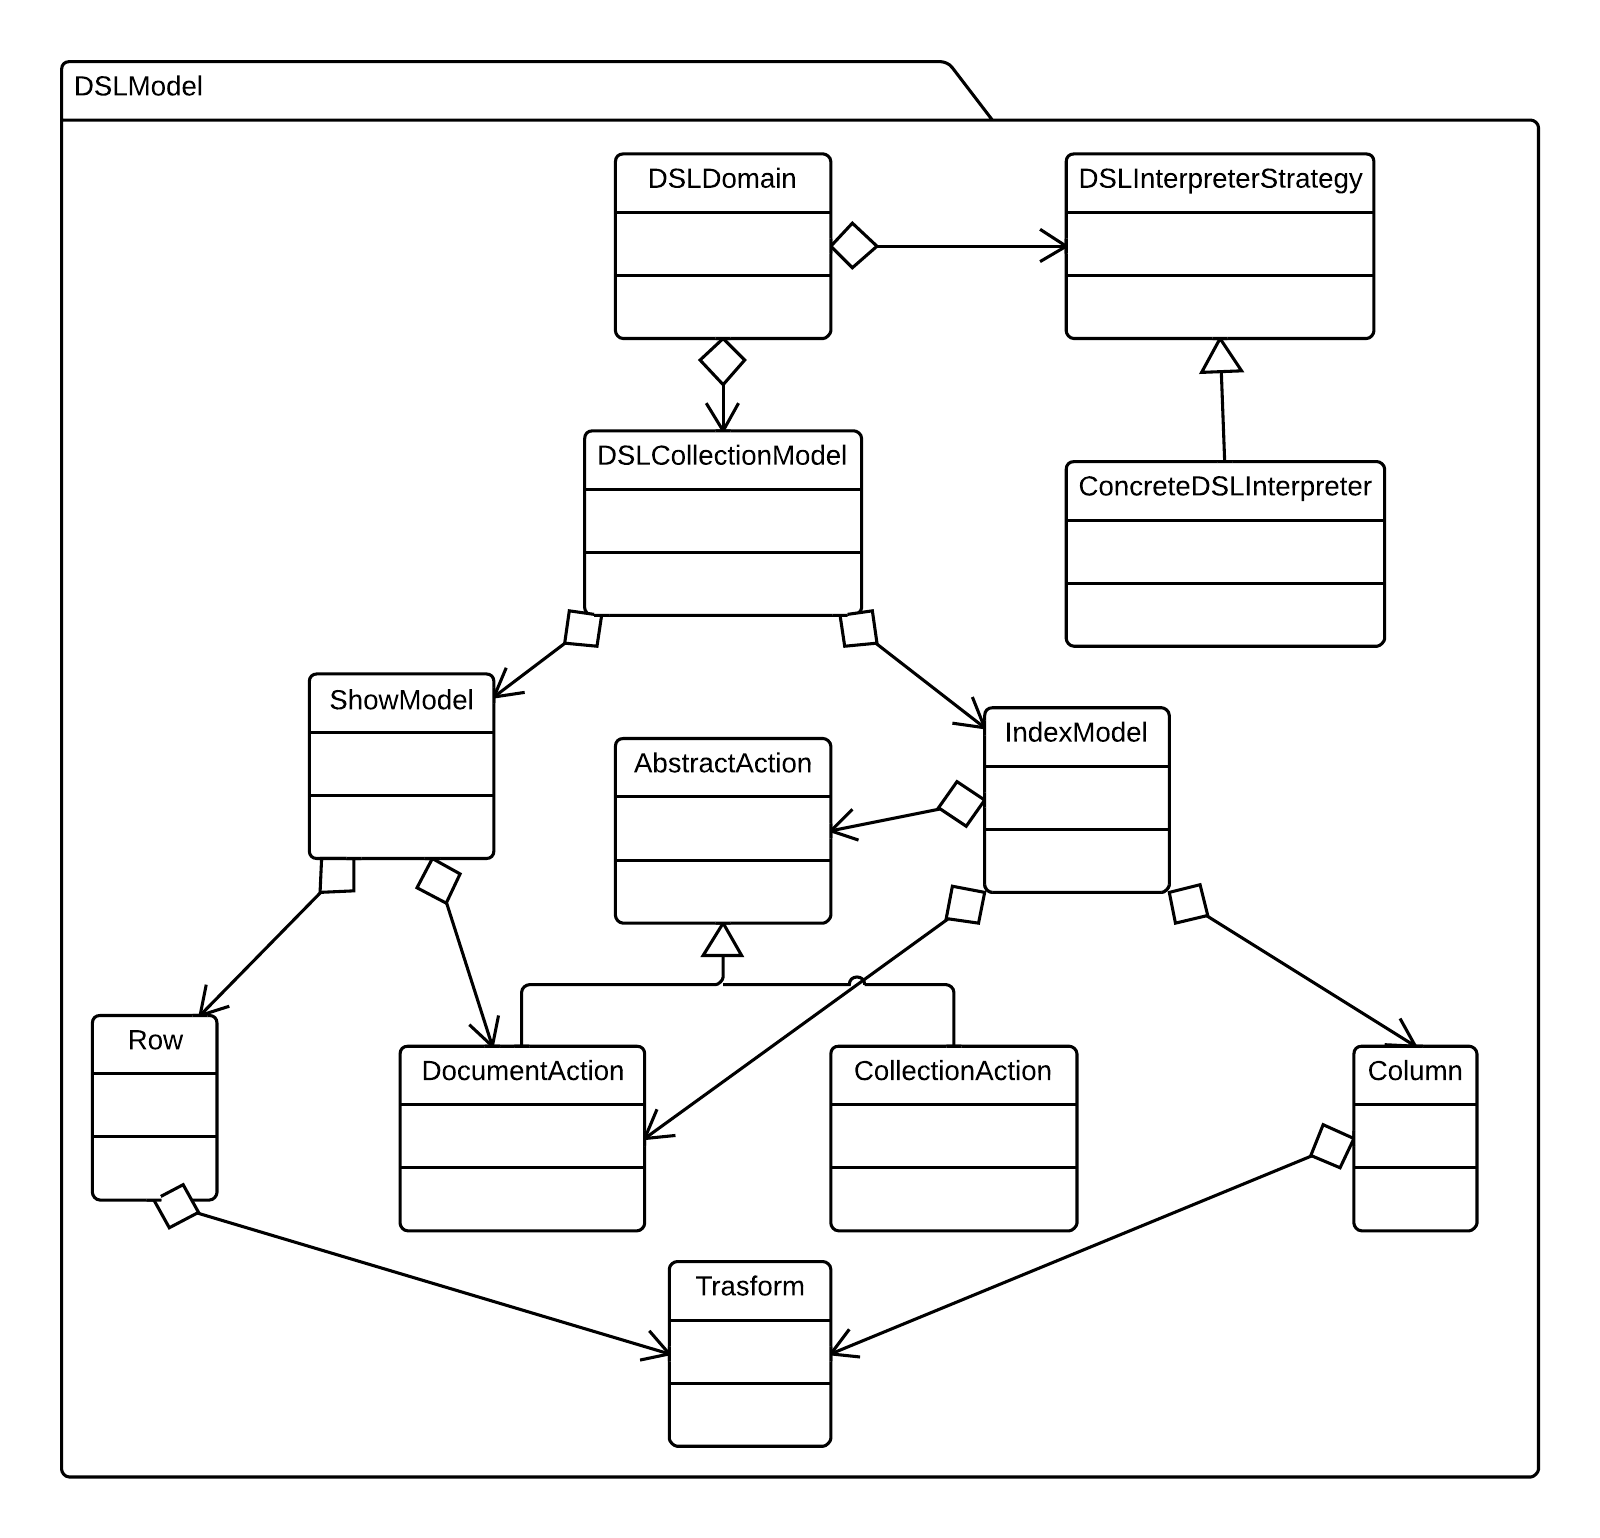
\includegraphics[width=\textwidth]{packages/Back-end::Lib::DSLModel.png}  
        \caption{Componente Back-end::Lib::DSLModel}
      \end{center}  
    \end{figure} 
  \subparagraph{Descrizione} 
    \begin{itemize}
    \item[] \glossario{Package} costituito da classi per la definizione delle regole di business sui dati definite tramite il \glossario{DSL}. 
Il \glossario{package} contiene principalmente classi che si occupano del caricamento del \glossario{DSL} e della sua rappresentazione in un modello ad oggetti. \\
Costituisce la componente model dell'architettura MVC del back-end.
    \end{itemize} 
    \paragraph{Classi}
      \subparagraph{Back-end::Lib::DSLModel::Column}
        
        \textbf{\\ \\ Descrizione} 
          \begin{itemize}
            \item[] 
          \end{itemize}      
        \textbf{Utilizzo}  
          \begin{itemize}
            \item[] 
          \end{itemize}
          \textbf{Relazioni con altre classi}
          \begin{itemize}
              \item{Back-end::Lib::DSLModel::Trasform}
          \end{itemize}
      \subparagraph{Back-end::Lib::DSLModel::DSLDomain}
        
        \textbf{\\ \\ Descrizione} 
          \begin{itemize}
            \item[] Classe che si occupa di caricare i file \glossario{DSL}. Implementa il \glossario{Design Pattern} \glossario{registry}.
          \end{itemize}      
        \textbf{Utilizzo}  
          \begin{itemize}
            \item[] Viene utilizzata per caricare dinamicamente tutti i \glossario{DSL} a partire dal \glossario{database} che le viene passato.
          \end{itemize}
          \textbf{Relazioni con altre classi}
          \begin{itemize}
              \item{Back-end::Lib::DSLModel::DSLInterpreterStrategy}
              \item{Back-end::Lib::DSLModel::DSLCollectionModel}
          \end{itemize}
      \subparagraph{Back-end::Lib::DSLModel::AbstractAction}
        
        \textbf{\\ \\ Descrizione} 
          \begin{itemize}
            \item[] 
          \end{itemize}      
        \textbf{Utilizzo}  
          \begin{itemize}
            \item[] 
          \end{itemize}
          \textbf{Classi Figlie}
          \begin{itemize}
              \item{Back-end::Lib::DSLModel::AbstractAction::CollectionAction}
              \item{Back-end::Lib::DSLModel::AbstractAction::DocumentAction}
          \end{itemize}
      \subparagraph{Back-end::Lib::DSLModel::ShowModel}
        
        \textbf{\\ \\ Descrizione} 
          \begin{itemize}
            \item[] 
          \end{itemize}      
        \textbf{Utilizzo}  
          \begin{itemize}
            \item[] 
          \end{itemize}
          \textbf{Relazioni con altre classi}
          \begin{itemize}
              \item{Back-end::Lib::DSLModel::Row}
          \end{itemize}
      \subparagraph{Back-end::Lib::DSLModel::IndexModel}
        
        \textbf{\\ \\ Descrizione} 
          \begin{itemize}
            \item[] 
          \end{itemize}      
        \textbf{Utilizzo}  
          \begin{itemize}
            \item[] 
          \end{itemize}
          \textbf{Relazioni con altre classi}
          \begin{itemize}
              \item{Back-end::Lib::DSLModel::AbstractAction::CollectionAction}
              \item{Back-end::Lib::DSLModel::AbstractAction::DocumentAction}
          \end{itemize}
      \subparagraph{Back-end::Lib::DSLModel::Row}
        
        \textbf{\\ \\ Descrizione} 
          \begin{itemize}
            \item[] 
          \end{itemize}      
        \textbf{Utilizzo}  
          \begin{itemize}
            \item[] 
          \end{itemize}
      \subparagraph{Back-end::Lib::DSLModel::AbstractAction::CollectionAction}
        
        \textbf{\\ \\ Descrizione} 
          \begin{itemize}
            \item[] 
          \end{itemize}      
        \textbf{Utilizzo}  
          \begin{itemize}
            \item[] 
          \end{itemize}
          \textbf{Classi Ereditate}
          \begin{itemize}
                \item{Back-end::Lib::DSLModel::AbstractAction}
          \end{itemize}
      \subparagraph{Back-end::Lib::DSLModel::AbstractAction::DocumentAction}
        
        \textbf{\\ \\ Descrizione} 
          \begin{itemize}
            \item[] 
          \end{itemize}      
        \textbf{Utilizzo}  
          \begin{itemize}
            \item[] 
          \end{itemize}
          \textbf{Classi Ereditate}
          \begin{itemize}
                \item{Back-end::Lib::DSLModel::AbstractAction}
          \end{itemize}
      \subparagraph{Back-end::Lib::DSLModel::Trasform}
        
        \textbf{\\ \\ Descrizione} 
          \begin{itemize}
            \item[] 
          \end{itemize}      
        \textbf{Utilizzo}  
          \begin{itemize}
            \item[] 
          \end{itemize}
      \subparagraph{Back-end::Lib::DSLModel::DSLInterpreterStrategy}
        
        \textbf{\\ \\ Descrizione} 
          \begin{itemize}
            \item[] Classe astratta che definisce l'interfaccia dell'algoritmo di interpretazione del linguaggio \glossario{DSL} utilizzato. È il componente strategy del \glossario{Design Pattern} \glossario{strategy}.
          \end{itemize}      
        \textbf{Utilizzo}  
          \begin{itemize}
            \item[] Viene utilizzata per incapsulare e rendere intercambiabile l'algoritmo di interpretazione del linguaggio \glossario{DSL}. In questo modo, se in futuro vi fosse necessità di cambiare l'algoritmo di interpretazione l'algoritmo può variare indipendentemente dal client che ne farà uso.
          \end{itemize}
          \textbf{Classi Figlie}
          \begin{itemize}
              \item{Back-end::Lib::DSLModel::DSLInterpreterStrategy::ConcreteDSLInterpreter}
          \end{itemize}
      \subparagraph{Back-end::Lib::DSLModel::DSLCollectionModel}
        
        \textbf{\\ \\ Descrizione} 
          \begin{itemize}
            \item[] Classe che si occupa di definire il model della \glossario{Collection} a partire dal \glossario{DSL}. Si ispira all'\glossario{Abstract Syntax Tree}.
          \end{itemize}      
        \textbf{Utilizzo}  
          \begin{itemize}
            \item[] È l'oggetto risultante dell'interpretazione del \glossario{DSL}. Definisce una rappresentazione interna di una \glossario{Collection}.
          \end{itemize}
          \textbf{Relazioni con altre classi}
          \begin{itemize}
              \item{Back-end::Lib::DSLModel::ShowModel}
              \item{Back-end::Lib::DSLModel::IndexModel}
          \end{itemize}
      \subparagraph{Back-end::Lib::DSLModel::DSLInterpreterStrategy::ConcreteDSLInterpreter}
        
        \textbf{\\ \\ Descrizione} 
          \begin{itemize}
            \item[] Classe che concretizza l'interprete del \glossario{DSL}. È uno dei componenti ConcreteStrategy del \glossario{Design Pattern} \glossario{Strategy}.
          \end{itemize}      
        \textbf{Utilizzo}  
          \begin{itemize}
            \item[] Viene utilizzata per implementare l'algoritmo utilizzato nell'interfaccia \texttt{Back-end::Lib::DSLModel::DSLInterpreterStrategy} per l'interpretazione del linguaggio \glossario{DSL}. Conterrà al suo interno un metodo che genererà il \glossario{parser} a partire da una grammatica regolare.
          \end{itemize}
          \textbf{Classi Ereditate}
          \begin{itemize}
                \item{Back-end::Lib::DSLModel::DSLInterpreterStrategy}
          \end{itemize}
  \subsubsection{Back-end::Lib::Controller}
  \paragraph{Informazioni sul package} 
    \begin{figure}[H] 
      \begin{center} 
        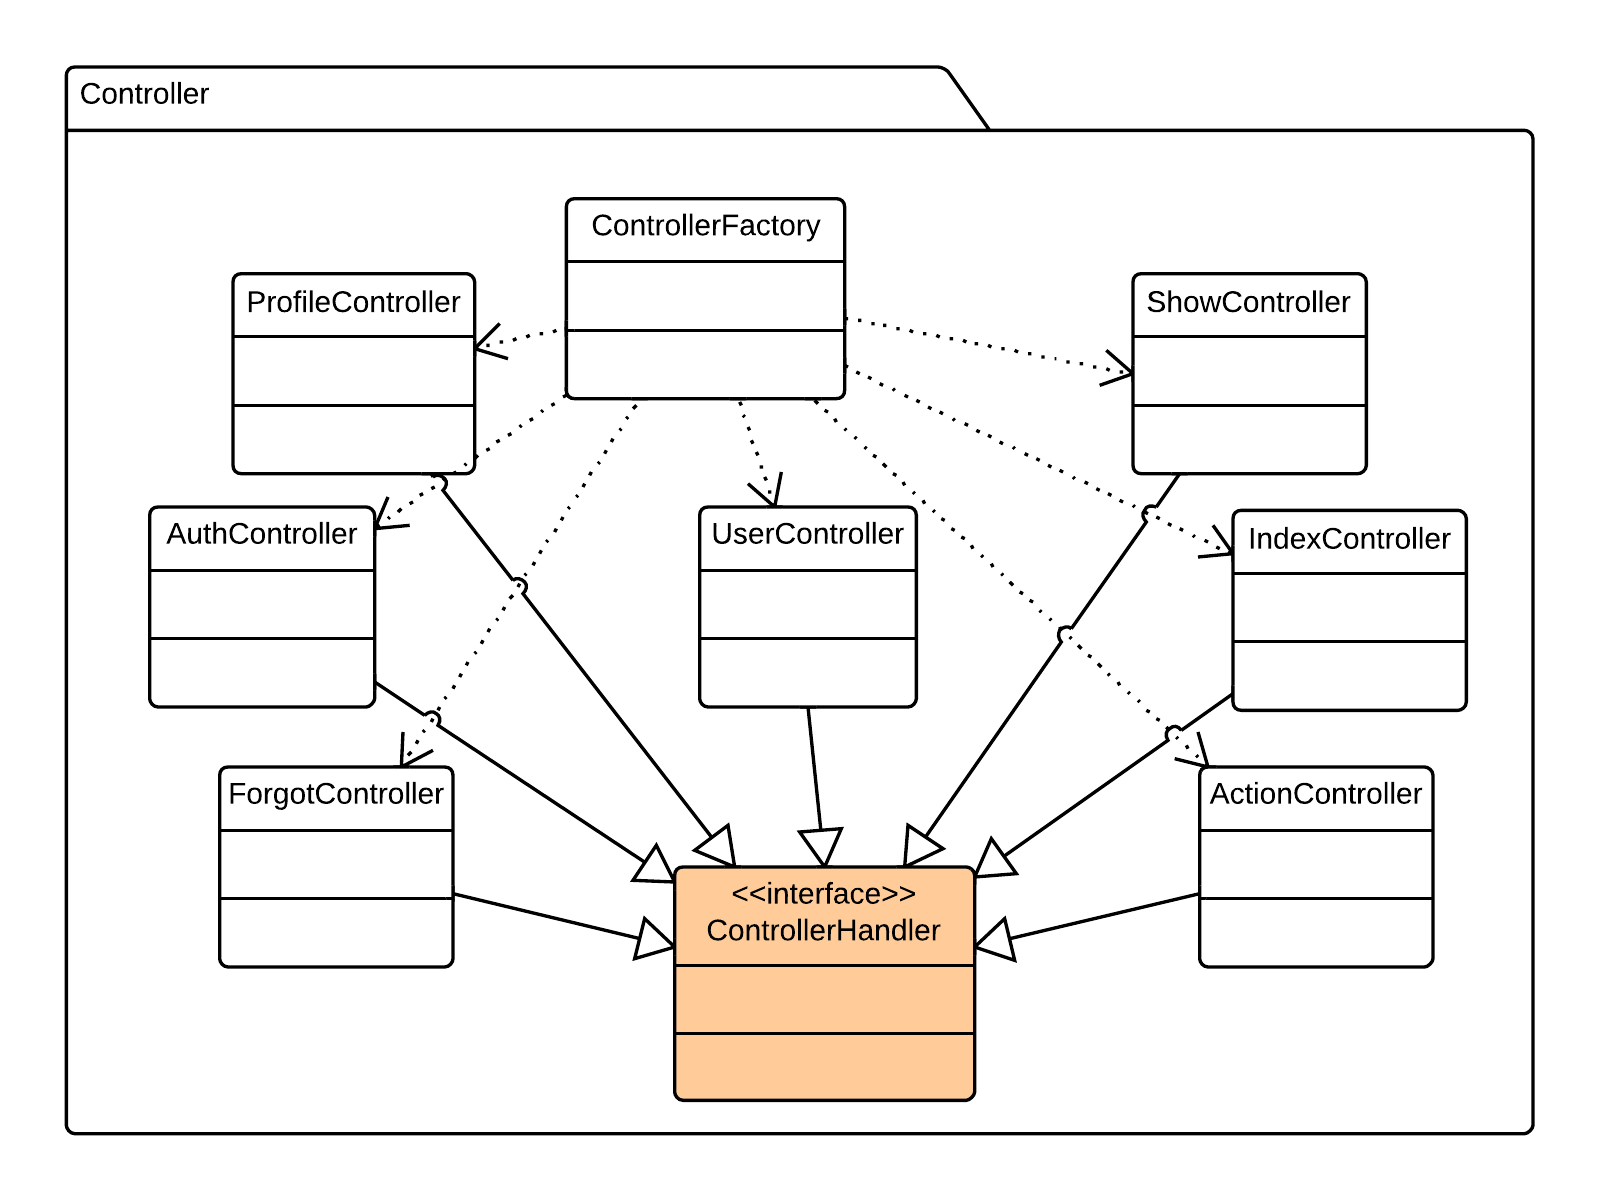
\includegraphics[width=\textwidth]{packages/Back-end::Lib::Controller.png}  
        \caption{Componente Back-end::Lib::Controller}
      \end{center}  
    \end{figure} 
  \subparagraph{Descrizione} 
    \begin{itemize}
    \item[] \glossario{Package} per il componente che realizza parte dell'application logic nell'architettura mvc nel back-end. Contiene classi per le funzionalità di controllo e visualizzazione delle risorse, dove ogni classe gestisce in modo esclusivo una sola di queste, in base all' \glossario{URI}.
    \end{itemize} 
    \paragraph{Classi}
      \subparagraph{Back-end::Lib::Controller::UserController}
        
        \textbf{\\ \\ Descrizione} 
          \begin{itemize}
            \item[] Classe che si occupa della varie operazioni che l'admin può compiere sugli utenti dell'applicazione. È uno dei componenti product del \glossario{Design Pattern} \glossario{Factory method}.
          \end{itemize}      
        \textbf{Utilizzo}  
          \begin{itemize}
            \item[] Viene utilizzata per visualizzare la \glossario{index-page} degli utenti, visualizzare le relative \glossario{show-page}, eliminare un utente e modificare il profilo. Mette a disposizione dei metodi per effettuare tutte queste operazioni.
          \end{itemize}
      \subparagraph{Back-end::Lib::Controller::ActionController}
        
        \textbf{\\ \\ Descrizione} 
          \begin{itemize}
            \item[] Classe che rappresenta i metodi per la gestione della risorsa corrispondente ad un'azione. 
È uno dei componenti product del \glossario{Design Pattern} \glossario{Factory method}.
          \end{itemize}      
        \textbf{Utilizzo}  
          \begin{itemize}
            \item[] Viene utilizzata per gestire le azioni personalizzate predisposte nelle pagine index-page e show-page, delegando alla classe \texttt{Back-end::Lib::DSLModel::DSLDomain} la loro esecuzione avendo quest'ultima l'implementazione delle stesse. 
          \end{itemize}
      \subparagraph{Back-end::Lib::Controller::ControllerFactory}
        
        \textbf{\\ \\ Descrizione} 
          \begin{itemize}
            \item[] Classe che si occupa di istanziare e restituire una classe \textit{Controller}. Rappresenta il componente creator del \glossario{Design Pattern} \glossario{Factory method}.
          \end{itemize}      
        \textbf{Utilizzo}  
          \begin{itemize}
            \item[] Viene costruita una sola volta dalla classe \texttt{Back-end::Lib::Middleware::Router} e si occupa di creare e restituire l'oggetto \textit{Controller} richiesto.
          \end{itemize}
      \subparagraph{Back-end::Lib::Controller::AuthController}
        
        \textbf{\\ \\ Descrizione} 
          \begin{itemize}
            \item[] Classe che rappresenta i metodi per la gestione delle risorse di login e logout. È uno dei componenti product del \glossario{Design Pattern} \glossario{Factory method}.

          \end{itemize}      
        \textbf{Utilizzo}  
          \begin{itemize}
            \item[] Viene utilizzata per gestire i dati di e le operazioni relativi all'autenticazione utente e al suo logout dall'applicazione, occupandosi della creazione della sessione utente e della sua distruzione tramite \glossario{cookies}.
          \end{itemize}
      \subparagraph{Back-end::Lib::Controller::ProfileController}
        
        \textbf{\\ \\ Descrizione} 
          \begin{itemize}
            \item[] Classe che rappresenta la gestione di un profilo utente. È uno dei componenti product del \glossario{Design Pattern} \glossario{Factory method}.
          \end{itemize}      
        \textbf{Utilizzo}  
          \begin{itemize}
            \item[] Viene utilizzata per visualizzare il profilo dell'utente, tramite GET, e per editarlo tramite PUT.
          \end{itemize}
      \subparagraph{Back-end::Lib::Controller::ShowController}
        
        \textbf{\\ \\ Descrizione} 
          \begin{itemize}
            \item[] Classe che si occupa della gestione della risorsa show-page.
È uno dei componenti product del \glossario{Design Pattern} \glossario{Factory method}.
          \end{itemize}      
        \textbf{Utilizzo}  
          \begin{itemize}
            \item[] Viene utilizzata per gestire una richiesta della risorsa show-page, delegando alla classe \texttt{Back-end::Lib::DSLModel::DSLDomain} la sua visualizzazione.
          \end{itemize}
      \subparagraph{Back-end::Lib::Controller::IndexController}
        
        \textbf{\\ \\ Descrizione} 
          \begin{itemize}
            \item[] Classe di gestione per la risorsa index 
È uno dei componenti product del \glossario{Design Pattern} \glossario{Factory method}.

          \end{itemize}      
        \textbf{Utilizzo}  
          \begin{itemize}
            \item[] Viene utilizzata per gestire la risorsa corrispondente all'index-page di un \glossario{Document}, offrendo metodi per restituirne gli attributi, effettuarne la modifica o la cancellazione e delega la visualizzazione dell'index-page alla classe \texttt{Back-end::Lib::DSLModel::DSLDomain}.

          \end{itemize}
      \subparagraph{Back-end::Lib::Controller::ForgotController}
        
        \textbf{\\ \\ Descrizione} 
          \begin{itemize}
            \item[] Classe che rappresenta il sistema di recupero e ripristino password. È uno dei componenti product del \glossario{Design Pattern} \glossario{Factory method}.
          \end{itemize}      
        \textbf{Utilizzo}  
          \begin{itemize}
            \item[] La classe fornisce dei metodi per effettuare una richiesta di reset password e, in un secondo momento, procedere al suo ripristino. La richiesta di reset avviene mandando un'email all'indirizzo dell'utente tramite la classe \texttt{Back-end::Lib::Middleware::Mailer}. All'interno di questo messaggio sarà presente un link che procederà ad effettuare il login dell'utente e a reindirizzarlo nella pagina di modifica profilo, dalla quale potrà modificare la password.
          \end{itemize}